% !TEX program = xelatex
\documentclass[12pt, a4paper]{book}

%---------------------------------------------------
% Page Layout and Margins (geometry package)
%---------------------------------------------------
\usepackage[
a4paper,
twoside,  % فعال‌سازی چیدمان دوطرفه برای کتاب
top=2.5cm,
bottom=3cm,
inner=3cm,  % حاشیه داخلی (سمت صحافی) - باید بزرگتر باشد
outer=2cm,  % حاشیه خارجی
headheight=14.5pt, % فضایی برای سرصفحه، برای جلوگیری از اخطار
% showframe  % <<< برای مشاهده بصری کادرها (در نسخه نهایی حذف شود)
]{geometry}


%---------------------------------------------------
% Main Packages
%---------------------------------------------------
\usepackage{amsmath}
\usepackage{amsfonts}
\usepackage{graphicx}

%---------------------------------------------------
% Algorithm and Pseudocode Packages
%---------------------------------------------------
\usepackage{algorithm}
\usepackage[noend]{algpseudocode} 

%---------------------------------------------------
% TikZ package for drawing graphs
%---------------------------------------------------
\usepackage{tikz}
\usetikzlibrary{arrows.meta, positioning, graphs, shapes.arrows}

%---------------------------------------------------
% Title Formatting Package
%---------------------------------------------------
\usepackage{titlesec}
% Define a custom length for title separation
\newcommand{\mytitlesep}{4pt} % مقدار فاصله به درخواست شما تغییر کرد

% Configuration for section titles using the custom length
\titleformat{\section}{\normalfont\Large\bfseries}{\thesection)}{\mytitlesep}{}
\titleformat{\subsection}{\normalfont\large\bfseries}{\thesubsection)}{\mytitlesep}{}
\titleformat{\subsubsection}{\normalfont\normalsize\bfseries}{\thesubsubsection)}{\mytitlesep}{}

% Modern package for caption control and fixing hyperlink targets
\usepackage{caption}
\captionsetup{hypcap=true}

%---------------------------------------------------
% Hyperlink package
%---------------------------------------------------
\usepackage[colorlinks=true, allcolors=blue]{hyperref}

%---------------------------------------------------
% Farsi language support (MUST be loaded last)
%---------------------------------------------------
\usepackage{xepersian}

%---------------------------------------------------
% Font Definitions
%---------------------------------------------------
\settextfont{XB Niloofar}
\setlatintextfont{Times New Roman}

%---------------------------------------------------
% Custom environment for LTR pseudocode
%---------------------------------------------------
\newenvironment{pseudocode}{%
	\begin{latin}
		\begin{algorithmic}[1]
		}{%
		\end{algorithmic}
	\end{latin}
}
\renewcommand{\algorithmicrequire}{\textbf{Input:}}
\renewcommand{\algorithmicensure}{\textbf{Output:}}


%---------------------------------------------------
% Document Information
%---------------------------------------------------
\title{درس‌نامه الگوریتم‌های گراف}
\author{
	نویسنده: محمد جواد عبدالهی
	\\ \\
	\large{با نظارت: دکتر بهناز عمومی}
}
\date{\today}


\begin{document}
	\setcounter{chapter}{-1} % This line starts chapter numbering from 0
	
	\maketitle
	\tableofcontents
	
	% Include chapters from separate files
	\chapter{مفاهیم پایه و تعاریف}
\label{chap:basics}

در این فصل، مفاهیم و تعاریف اولیه‌ای که در سراسر این جزوه به آن‌ها نیاز خواهیم داشت را مرور می‌کنیم.

\section{تعریف گراف}
\label{def:graph}
به طور رسمی، یک \textbf{گراف} $G$ یک سه‌تایی مرتب $G=(V, E, \psi)$ است که در آن:
\begin{itemize}
	\item $V$ یک مجموعه متناهی و ناتهی از عناصر به نام \textbf{رئوس} (\lr{Vertices}) است.
	\item $E$ یک مجموعه متناهی (و مجزا از $V$) از عناصر به نام \textbf{یال‌ها} (\lr{Edges}) است.
	\item $\psi$ یک \textbf{تابع وقوع} (\lr{incidence function}) است که هر یال را به یک زوج (نامرتب) از رئوس نگاشت می‌دهد.
\end{itemize}

\subsection{طوقه (\lr{Loop})}
اگر برای یک یال $e$، دو سر آن یکسان باشند، یعنی $\psi(e) = \{u, u\}$، آنگاه $e$ را یک \textbf{طوقه} می‌نامیم.
\begin{figure}[H]
	\centering
	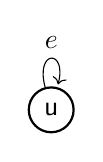
\begin{tikzpicture}[vertex/.style={draw, circle, thick, font=\sffamily}]
		\node[vertex] (u) at (0,0) {u};
		\path (u) edge [loop above] node[above] {$e$} (u);
	\end{tikzpicture}
	\caption{نمایش یک طوقه $e$ روی رأس $u$.}
\end{figure}

\subsection{یال‌های موازی (\lr{Parallel Edges})}
اگر دو یال مختلف $e_1$ و $e_2$ دو سر یکسانی داشته باشند، آن دو را \textbf{یال‌های موازی} می‌گوییم.
\begin{figure}[H]
	\centering
	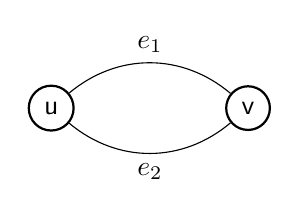
\begin{tikzpicture}[vertex/.style={draw, circle, thick, font=\sffamily}]
		\node[vertex] (u) at (0,0) {u};
		\node[vertex] (v) at (2.5,0) {v};
		\path (u) edge [bend left=40] node[above] {$e_1$} (v)
		(u) edge [bend right=40] node[below] {$e_2$} (v);
	\end{tikzpicture}
	\caption{نمایش دو یال موازی بین رئوس $u$ و $v$.}
\end{figure}

\subsection{گراف ساده (\lr{Simple Graph})}
گرافی که هیچ طوقه و یال موازی نداشته باشد، \textbf{گراف ساده} نامیده می‌شود.

\subsection{گراف جهت‌دار (\lr{Directed Graph})}
در \textbf{گراف جهت‌دار}، تابع وقوع هر یال را به یک \textbf{زوج مرتب} از رئوس نگاشت می‌دهد: $\psi: E \to (V \times V)$.

\section{نمایش گراف در کامپیوتر}
\label{sec:graph_representation}
برای پیاده‌سازی الگوریتم‌های گراف، باید گراف را به شیوه‌ای کارآمد در حافظه کامپیوتر ذخیره کنیم. دو روش متداول برای این کار ماتریس مجاورت و لیست مجاورت هستند.

\subsection{ماتریس مجاورت (\lr{Adjacency Matrix})}
یک ماتریس $n \times n$ (که $n = |V|$) به نام $A$ است که در آن درایه $A_{ij}$ برابر ۱ است اگر یالی بین رأس $i$ و رأس $j$ وجود داشته باشد و در غیر این صورت برابر ۰ است. این روش برای گراف‌های متراکم کارآمد است.

\subsection{لیست مجاورت (\lr{Adjacency List})}
\label{def:adj_list}
یک آرایه از لیست‌ها به اندازه $n$ است که در آن، خانه $i$-ام آرایه، لیستی از همسایگان رأس $i$ را نگهداری می‌کند. این روش برای گراف‌های خلوت (که تعداد یال‌ها بسیار کمتر از $n^2$ است) بسیار بهینه‌تر است.

\begin{figure}[H]
	\centering
	\begin{tikzpicture}[vertex/.style={draw, circle, thick, font=\sffamily}, scale=0.9, every node/.style={scale=0.9}]
		\node[vertex] (1) at (0, 1.5) {1};
		\node[vertex] (2) at (-1.5, 0) {2};
		\node[vertex] (3) at (1.5, 0) {3};
		\path[-, thick] (1) edge (2) (1) edge (3) (2) edge (3);
		\node at (0, -1) {(a) گراف نمونه};
		
		\begin{scope}[xshift=5cm]
			\node[draw, minimum width=1cm] (l1) at (0, 2) {1};
			\node[draw, minimum width=1cm] (l2) at (0, 1) {2};
			\node[draw, minimum width=1cm] (l3) at (0, 0) {3};
			\path[->, thick] (l1) edge (1,2); \node[draw] at (1.5,2) {2}; \path[->, thick] (1.5,2) edge (2.5,2); \node[draw] at (3,2) {3};
			\path[->, thick] (l2) edge (1,1); \node[draw] at (1.5,1) {1}; \path[->, thick] (1.5,1) edge (2.5,1); \node[draw] at (3,1) {3};
			\path[->, thick] (l3) edge (1,0); \node[draw] at (1.5,0) {1}; \path[->, thick] (1.5,0) edge (2.5,0); \node[draw] at (3,0) {2};
			\node at (1.5, -1) {(b) نمایش با لیست مجاورت};
		\end{scope}
	\end{tikzpicture}
	\caption{یک گراف و نمایش آن با لیست مجاورت.}
\end{figure}

\section{صف (\lr{Queue})}
\label{def:queue}
یک \textbf{صف} یک ساختمان داده خطی است که از اصل \textbf{ورودی اول، خروجی اول} (\lr{First-In, First-Out - FIFO}) پیروی می‌کند. دو عمل اصلی روی صف عبارتند از:
\begin{itemize}
	\item \textbf{\lr{Enqueue}:} افزودن یک عنصر به \textbf{انتهای} صف (\lr{Rear}).
	\item \textbf{\lr{Dequeue}:} حذف یک عنصر از \textbf{ابتدای} صف (\lr{Front}).
\end{itemize}
این رفتار در شکل \ref{fig:queue_diagram} به صورت گرافیکی نمایش داده شده است.

\begin{figure}[H]
	\centering
	\begin{tikzpicture}[
		box/.style={draw, thick, minimum width=1.2cm, minimum height=1.2cm, font=\Large},
		arrow/.style={single arrow, draw, thick, single arrow head extend=5pt}
		]
		\node[box] (q1) at (0,0) {A};
		\node[box] (q2) at (1.2,0) {B};
		\node[box] (q3) at (2.4,0) {C};
		\node[above=3mm of q1] (front) {جلو \lr{(Front)}};
		\node[above=3mm of q3] (rear) {عقب \lr{(Rear)}};
		\node[arrow, fill=red!20, minimum height=1.5cm, rotate=-90] at (0, -1.2) {};
		\node[below=1.25cm of q1] {\lr{Dequeue}};
		\node[arrow, fill=green!20, minimum height=1.5cm, rotate=-180] at (4, 0) {};
		\node[] at (4,-0.6) {\lr{Enqueue}};
	\end{tikzpicture}
	\caption{نمایش گرافیکی یک صف و عملیات اصلی آن.}
	\label{fig:queue_diagram}
\end{figure}
	\chapter{تکنیک‌های اولیه پیمایش گراف}
\label{chap:traversal}

پس از آشنایی با تعاریف رسمی گراف در فصل قبل، در این فصل به سراغ دو روش بنیادین برای پیمایش رئوس و یال‌های گراف می‌رویم: جستجوی اول سطح (\lr{BFS}) و جستجوی اول عمق (\lr{DFS}). این الگوریتم‌ها سنگ بنای بسیاری از الگوریتم‌های پیشرفته‌تر گراف هستند. ما در این بخش، این الگوریتم‌ها را عمدتاً روی \textbf{گراف‌های ساده} توضیح می‌دهیم، اما منطق آن‌ها با استفاده از نمایش \textbf{لیست مجاورت} (\lr{Adjacency List}) (بخش \ref{def:adj_list})، برای گراف‌های دارای یال موازی نیز قابل تعمیم است.

\section{جستجوی اول سطح (\lr{Breadth-First Search - BFS})}
\label{sec:bfs}

الگوریتم جستجوی اول سطح (\lr{BFS}) یکی از ساده‌ترین و در عین حال پرکاربردترین الگوریتم‌های پیمایش گراف است. ایده اصلی این الگوریتم، شروع از یک رأس مبدأ و کاوش گراف به صورت لایه به لایه است.

\subsection{توضیح الگوریتم}
الگوریتم \lr{BFS} از یک رأس مشخص (مبدأ یا \lr{s}) شروع به پیمایش می‌کند و فرض می‌کند گراف با یک نمایش مناسب مانند \textbf{لیست مجاورت} (\lr{Adjacency List}) داده شده است. الگوریتم ابتدا تمام همسایه‌های مستقیم رأس \lr{s} را ملاقات می‌کند (لایه اول) و این روند را تا زمانی که تمام رئوس قابل دسترس از \lr{s} ملاقات شوند، ادامه می‌دهد. برای پیاده‌سازی این رفتار "لایه به لایه"، الگوریتم از یک \textbf{صف} (\lr{Queue}) (بخش \ref{def:queue}) استفاده می‌کند.

\subsection{شبه‌کد الگوریتم}
\begin{algorithm}[H]
	\caption{Breadth-First Search (BFS)}
	\label{alg:bfs}
	\begin{pseudocode}
		\Procedure{BFS}{$G, s$}
		\State Let $Q$ be a queue
		\State $Q$.enqueue($s$)
		\State Mark $s$ as visited
		\While{$Q$ is not empty}
		\State $u \gets Q$.dequeue()
		\State Process $u$ (e.g., print it)
		\For{each neighbor $v$ of $u$}
		\If{$v$ has not been visited}
		\State Mark $v$ as visited
		\State $Q$.enqueue($v$)
		\EndIf
		\EndFor
		\EndWhile
		\EndProcedure
	\end{pseudocode}
\end{algorithm}

\subsection{مثال}
یک گراف ساده و بدون جهت مانند شکل \ref{fig:bfs_example_graph} را در نظر بگیرید. می‌خواهیم پیمایش \lr{BFS} را از رأس \lr{A} شروع کنیم.
\begin{figure}[H]
	\centering
	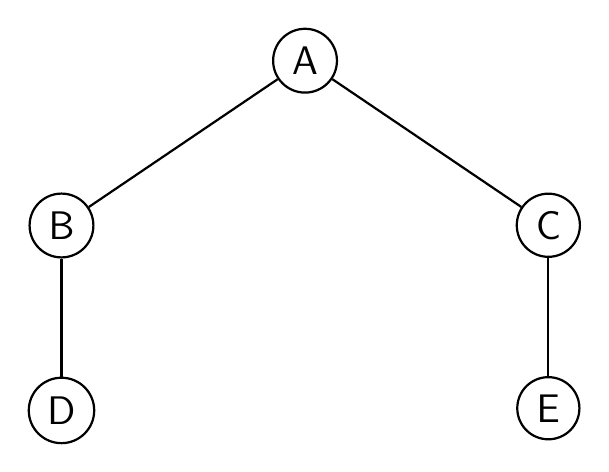
\begin{tikzpicture}[
		node distance=1.5cm and 2.5cm,
		every node/.style={draw, circle, thick, font=\sffamily\Large}
		]
		\node (A) {A};
		\node (B) [below left=of A] {B};
		\node (C) [below right=of A] {C};
		\node (D) [below=of B] {D};
		\node (E) [below=of C] {E};
		\path[-, thick]
		(A) edge (B) (A) edge (C) (B) edge (D) (C) edge (E);
	\end{tikzpicture}
	\caption{یک گراف ساده و بدون جهت برای پیمایش \lr{BFS} از رأس \lr{A}.}
	\label{fig:bfs_example_graph}
\end{figure}
ترتیب ملاقات رئوس: \textbf{\lr{A, B, C, D, E}}.

\subsection{انیمیشن و ابزارهای پایتون}
\begin{itemize}
	\item \textbf{انیمیشن آنلاین:} برای درک شهودی، انیمیشن‌های تعاملی روند اجرای \lr{BFS} را در وب‌سایت \href{https://visualgo.net/en/dfsbfs}{Visualgo} مشاهده کنید.
	\item \textbf{اسکریپت پایتون تعاملی:} در کنار این جزوه، فایلی به نام \lr{bfs\_animation.py} قرار دارد. با اجرای این اسکریپت، می‌توانید روند اجرای الگوریتم \lr{BFS} را روی یک گراف نمونه به صورت یک انیمیشن مشاهده کنید. این اسکریپت از کتابخانه‌های \lr{\texttt{networkx}} برای منطق گراف و \lr{\texttt{matplotlib}} برای تولید انیمیشن استفاده می‌کند.
\end{itemize}
	% \include{chapter2}
	% ... and so on
	
\end{document}